% PAPER_BTFR_MNRAS --- standalone observational article targeting MNRAS / A&A.
%
% Densified, self-contained rewrite of the former "Paper IV". Design goals,
% set by the editorial diagnosis of the CQG desk rejection:
%   (1) MINIMAL framework dependence. The paper is a test of a single,
%       falsifiable modified-gravity hypothesis (a0 propto H(z)). The originating
%       causal-network theory is cited once as provenance and never again relied
%       upon; an editor/referee can evaluate the entire paper without accepting
%       it. This removes the "theory-of-everything manifesto" desk-reject trigger.
%   (2) STEP-BY-STEP rigour. Every equation is derived line by line; the full
%       statistical machinery (error model, systematic floor, significance
%       estimator, forecast ceiling, null-exclusion) is written out, not asserted.
%   (3) HONEST assessment of validity. The result is reported as "evidence
%       consistent with, not confirmation of" the prediction, with the open
%       tensions (slope form; mass-axis discordance) stated in the same place as
%       the positive result. This is exactly what the CQG letter asked for.
%
% Compiles with pdflatex + bibtex against the shared TEIC_CONSOLIDATED.bib.
% Figures reused from the paper_IV build. At submission this converts to the
% mnras / aa class; the article-class build here is for review and page count.
\documentclass[fleqn,usenatbib]{mnras}
\usepackage[T1]{fontenc}
\usepackage{amsmath,amssymb}
\usepackage{mathptmx} % Times New Roman (text + math) for MNRAS house style
\usepackage{graphicx}
\usepackage{booktabs}
\usepackage{array}
\usepackage{hyperref}
\graphicspath{{paper_IV/figures/}{figures/}}

\newcommand{\dlogv}{\Delta\log_{10} v_{\rm flat}}
\newcommand{\azero}{a_0}
\newcommand{\sgal}{\sigma_{\rm gal}}
\newcommand{\ssys}{\sigma_{\rm sys}}

\title[Does the radial-acceleration scale evolve?]{Does the
radial-acceleration scale evolve? A pre-registered test of
$a_0\propto H(z)$ with the baryonic Tully--Fisher relation,
and first constraints at $z\sim1$}
\author[M. A. Mendes]{Miqueias Alves Mendes$^{1}$\thanks{E-mail:
mendes.eng.proj@gmail.com}\\
$^{1}$Independent Researcher, Ibiapina, Cear\'a, Brazil}
\date{Submitted 2026}
\pubyear{2026}

\begin{document}
\maketitle

\begin{abstract}
The radial acceleration relation (RAR) of disc galaxies is set by a scale
$\azero\simeq1.2\times10^{-10}\,{\rm m\,s^{-2}}$. In cold-dark-matter galaxy
formation it is an emergent constant, so the RAR and baryonic Tully--Fisher
relation ($v_{\rm flat}^4=GM_b\azero$) should not evolve at fixed $M_b$. A class of
modified-dynamics theories instead ties $\azero$ to the cosmic expansion,
$\azero(z)=\azero(0)\,H(z)/H_0$; one such theory (from a causal-network framework)
is described elsewhere, but the test here is independent of it. With the cosmology
fixed it predicts, parameter-free, $\dlogv(z)=\tfrac14\log_{10}[H(z)/H_0]$ at fixed
$M_b$, against a null of zero evolution. Before kinematic data beyond $z\sim0.3$
existed we pre-registered a protocol: selection criteria isolating the
low-acceleration regime, a two-component error model separating a per-galaxy
statistical term from a non-averaging systematic floor $\ssys$, a forecast, and a
verbatim kill criterion. The forecast shows the test is \emph{systematics}-limited:
at $z\sim1$ it saturates at $\approx1.5\sigma$ for $\ssys\approx0.04$~dex regardless
of sample size, decisive only at $z\ge2$ with $\ssys\le0.03$~dex. Applying the
unmodified protocol to the first qualifying public catalogue
(MUSE-DARK~III; 79 sub-maximal rotators at $0.33<z<1.44$), we measure
$\azero$ rising at $\ge15\sigma$, matching the prediction at $0.5$--$0.9\sigma$ on
the independent SPARC anchor, while a redshift-independent RAR is disfavoured at
$\sim19\sigma$. This is evidence consistent with, not confirmation of, the
prediction: the decisive $z\ge2$ regime is unmeasured, the functional form is
undecided ($2$--$3\sigma$ faster than $H$), and a same-epoch mass-axis analysis
finds no evolution. The kill criterion is armed; a second prediction
(Newtonian wide binaries below $\sim17$~pc) is exposed to Gaia.
\end{abstract}

\begin{keywords}
gravitation -- dark matter -- galaxies: kinematics and dynamics --
cosmology: observations
\end{keywords}

\section{Introduction}\label{sec:intro}

The tight empirical coupling between the observed centripetal acceleration in disc
galaxies, $g_{\rm obs}$, and the acceleration $g_{\rm bar}$ predicted from the
baryons alone---the radial acceleration relation
\citep{McGaugh2016,Lelli2016}---is one of the most regular scaling laws in
extragalactic astronomy. In the low-acceleration limit it takes the form
$g_{\rm obs}\to\sqrt{g_{\rm bar}\,\azero}$, with a single characteristic scale
$\azero\approx1.2\times10^{-10}\,{\rm m\,s^{-2}}$; integrated over a flat rotation
curve this is precisely the baryonic Tully--Fisher relation,
$v_{\rm flat}^4=G\,M_b\,\azero$ \citep{Milgrom1983,McGaugh2016}.

The \emph{interpretation} of $\azero$ divides current theories. In $\Lambda$CDM the
relation is emergent rather than fundamental: hydrodynamic simulations show that the
RAR arises naturally from galaxy formation in cold-dark-matter haloes, with feedback
shifting galaxies \emph{along} the relation rather than off
it~\citep{Ludlow2017}. We are careful not to overstate the resulting null: the
simplest expectation is a redshift-independent scale (since $\azero$ reflects slowly
varying combinations of the cosmic baryon fraction, halo concentration, and
disc-formation physics), but because feedback sets the scale, some galaxy-formation
models admit a \emph{mild} evolution whose amplitude and even sign depend on the
feedback prescription and are not yet converged across the IllustrisTNG, EAGLE, and
SIMBA suites. The $\Lambda$CDM ``null'' tested here is therefore the specific,
well-motivated hypothesis of a redshift-independent RAR, and we return to the
model-dependent simulation expectation in \S\ref{sec:robust}. A second, broad class
of modified-dynamics theories instead treats $\azero$ as a genuine acceleration scale
of the gravitational sector, and several of them tie it to the only acceleration the
background cosmology supplies, the Hubble rate, $\azero\sim cH$. Promoting this to an
evolution law,
\begin{equation}
\azero(z)=\azero(0)\,\frac{H(z)}{H_0},
\label{eq:a0z}
\end{equation}
turns a qualitative coincidence ($\azero\approx cH_0/2\pi$ today) into a
quantitative, falsifiable prediction: \emph{galaxies of fixed baryonic mass rotated
faster in the past}. One effective theory that produces Eq.~\eqref{eq:a0z}---a
scalar--vector--tensor layer derived from a discrete causal network---is described
elsewhere \citep{TEICDoc1}; we cite it only as the provenance of the hypothesis.
\emph{This paper does not depend on that derivation, on the causal-network theory, or
on any of its other ingredients: it tests only the observational hypothesis
$\azero\propto H(z)$, and the reader may regard Eq.~\eqref{eq:a0z} as a
parameter-free phenomenological ansatz to be confronted with data.} What makes the
confrontation informative is that the predicted evolution is a \emph{specific,
parameter-free} curve (\S\ref{sec:prediction}), sharper than the model-dependent
$\Lambda$CDM expectation: the data can exclude the redshift-independent null, can
match the specific $H(z)$ amplitude, or can do neither, and each outcome is
distinguishable.

The practical obstacle has never been the existence of the prediction but the
\emph{regime} in which it can be tested. The effect lives only where the dynamics
are modified, $g_{\rm obs}\lesssim\azero$; in baryon-dominated, high-surface-
brightness discs the predicted signal is intrinsically small and is swamped by
zero-point systematics. This is why pre-2026 high-redshift kinematics did not settle
the question (\S\ref{sec:kmos}). Accordingly, we treat the problem as a
pre-registered measurement: in \S\ref{sec:methods} we fix, in advance, the
sample-selection criteria (\S\ref{sec:selection}), the prediction and its derivation
(\S\ref{sec:prediction}), the statistical error model and significance estimator
(\S\ref{sec:stat}), a quantitative forecast of detectability
(\S\ref{sec:forecast}), and a verbatim kill criterion (\S\ref{sec:kill}). In
\S\ref{sec:results} we apply this protocol, unmodified, to the first public
catalogue that falls in the correct regime, MUSE-DARK~III \citep{Ciocan2026}.
\S\ref{sec:discussion} discusses what the result is and is not;
\S\ref{sec:wb} states a second, independent falsifiable prediction; and
\S\ref{sec:conclusions} concludes. Throughout we adopt a flat cosmology with
$\Omega_m=0.30\pm0.02$; as shown below, $H_0$ cancels from the observable.

\section{Methods (pre-registered)}\label{sec:methods}

\subsection{The prediction, derived}\label{sec:prediction}

We derive the observable from Eq.~\eqref{eq:a0z} and the BTFR with no hidden step.
In the low-acceleration regime the flat rotation speed obeys
\begin{equation}
v_{\rm flat}^4 = G\,M_b\,\azero .
\label{eq:btfr}
\end{equation}
Take the base-10 logarithm of both sides:
\begin{equation}
4\,\log_{10} v_{\rm flat} = \log_{10}(G\,M_b) + \log_{10}\azero .
\label{eq:logbtfr}
\end{equation}
Now compare two galaxies of \emph{identical} baryonic mass $M_b$, one at redshift
$z$ and one at $z=0$. The term $\log_{10}(GM_b)$ is common to both and cancels in
the difference, leaving
\begin{equation}
4\,\big[\log_{10} v_{\rm flat}(z)-\log_{10}v_{\rm flat}(0)\big]
= \log_{10}\azero(z)-\log_{10}\azero(0).
\label{eq:diff}
\end{equation}
Insert the evolution law Eq.~\eqref{eq:a0z}, for which
$\log_{10}\azero(z)-\log_{10}\azero(0)=\log_{10}[H(z)/H_0]$, and divide by four:
\begin{equation}
\boxed{\;\dlogv(z)=\tfrac14\,\log_{10}\!\left[\frac{H(z)}{H_0}\right]\;}
\label{eq:prediction}
\end{equation}
This is parameter-free once the cosmology is fixed. With
$H(z)/H_0=\sqrt{\Omega_m(1+z)^3+(1-\Omega_m)}$ and $\Omega_m=0.30$ it evaluates to
\begin{equation}
\dlogv = +0.061,\ +0.091,\ +0.118,\ +0.162~{\rm dex}
\label{eq:numbers}
\end{equation}
at $z=1,\,1.5,\,2,\,3$ respectively, where, e.g.\ at $z=1$,
$H/H_0=\sqrt{0.3\cdot8+0.7}=1.760$,
$\tfrac14\log_{10}1.760=0.0614$. The notable point is that $H_0$ has cancelled
identically (it appears only inside the ratio $H(z)/H_0$), so the prediction carries
no dependence on the Hubble-tension value of $H_0$; the only cosmological input is
the shape factor $\Omega_m$, which we propagate as a $\pm0.02$ band (this widens the
$z=1$ prediction by $\pm0.004$~dex, negligible against the systematic floor below).

\paragraph{Two equivalent axes.} Eq.~\eqref{eq:prediction} can be tested on the
\emph{velocity axis} (shift of the BTFR zero-point at fixed $M_b$) or, equivalently,
on the \emph{acceleration axis} (the value of $\azero$ recovered from a RAR fit),
through the one-to-one map
\begin{equation}
\azero(z)=\azero(0)\,\frac{H(z)}{H_0}
\;\Longleftrightarrow\;
\dlogv=\tfrac14\log_{10}\!\left[\frac{H(z)}{H_0}\right].
\label{eq:equiv}
\end{equation}
On the acceleration axis the prediction is a factor $H(1)/H_0=1.76$ rise in $\azero$
between $z=0$ and $z=1$, directly readable from any RAR fit of a low-acceleration
sample. We use the acceleration axis for the primary analysis because the public
catalogue reports a fitted $\azero(z)$; the mass-axis reading is discussed as an
independent cross-check in \S\ref{sec:notconfirm}.

\subsection{Sample-selection criteria}\label{sec:selection}

Because the effect exists only for $g_{\rm obs}\lesssim\azero$, we fix four
selection conditions in advance; a sample must satisfy all four to constitute a test
of Eq.~\eqref{eq:prediction}:
\begin{enumerate}
\item[(S1)] low baryonic/stellar mass (the low-acceleration end of the BTFR);
\item[(S2)] high gas fraction (so that $M_b$ is gas-dominated and less sensitive to
stellar mass-to-light systematics);
\item[(S3)] sub-maximal, dark-matter-dominated discs, placing the measured part of
the rotation curve in the regime $g_{\rm obs}\lesssim\azero$;
\item[(S4)] 3D kinematic modelling with pressure-support (asymmetric-drift)
corrections, so that $v_{\rm flat}$ is the dynamical circular speed, not the raw
line-of-sight velocity.
\end{enumerate}
Samples that violate (S1)--(S3)---massive, high-surface-brightness, baryon-dominated
discs in the high-acceleration (Newtonian) regime---are excluded \emph{a priori}:
there the predicted $\azero(z)$ signal is intrinsically weak and the formal velocity
errors are dominated by zero-point systematics (\S\ref{sec:kmos}). The selection,
not any particular catalogue, defines the ``correct regime''; it is a property of
the protocol.

\subsection{Error model and significance estimator}\label{sec:stat}

The observable is $\dlogv$ at fixed $M_b$ (equivalently $\Delta\log_{10}\azero$,
four times larger). We model the uncertainty on a binned measurement built from $N$
qualifying galaxies as the quadrature sum of two physically distinct components:
\begin{equation}
\sigma^2(N) = \frac{\sgal^2}{N} + \ssys^2 .
\label{eq:errormodel}
\end{equation}
The two terms behave oppositely with sample size and this is the crux of the whole
analysis:
\begin{itemize}
\item $\sgal\approx0.10$~dex is the \emph{per-galaxy statistical} scatter (velocity
measurement, inclination, individual mass estimate). It averages down as
$\sgal/\sqrt N$ and can be made arbitrarily small with a large enough sample.
\item $\ssys$ is the \emph{zero-point systematic floor}: the irreducible uncertainty
in the location of the $z=0$ anchor and in the cross-calibration of mass, beam
smearing, and pressure support between the high-$z$ sample and that anchor. It is
\emph{common} to all galaxies in a bin and therefore does \emph{not} average down;
it sets a ceiling on attainable significance.
\end{itemize}
The detection significance of a signal $\Delta(z)$ (Eq.~\ref{eq:numbers}) is
\begin{equation}
\mathcal{S}(N,z)=\frac{\Delta(z)}{\sigma(N)}
=\frac{\Delta(z)}{\sqrt{\sgal^2/N+\ssys^2}} ,
\label{eq:signif}
\end{equation}
whose large-$N$ limit is the \emph{ceiling significance}
\begin{equation}
\mathcal{S}_\infty(z)=\frac{\Delta(z)}{\ssys},
\label{eq:ceiling}
\end{equation}
independent of $N$. Inverting Eq.~\eqref{eq:signif} for the sample size required to
reach a target significance $\mathcal{S}_\star$ gives
\begin{equation}
N_\star(z)=\frac{\sgal^2}{\big[\Delta(z)/\mathcal{S}_\star\big]^2-\ssys^2},
\label{eq:Nstar}
\end{equation}
which diverges (no $N$ suffices) as $\Delta(z)/\mathcal{S}_\star\to\ssys$, i.e.\ once
the target exceeds the ceiling. Equations \eqref{eq:errormodel}--\eqref{eq:Nstar}
are the entire statistical engine; they are deliberately elementary so that the
result cannot hide in an estimator.

\paragraph{Anchor matrix.} The systematic floor is dominated by the choice of $z=0$
anchor, so we declare \emph{two independent} local anchors in advance and quote every
amplitude comparison against each:
\begin{equation}
\azero(0)=\begin{cases}
1.20\pm0.26 & \text{SPARC},\\[2pt]
1.69\pm0.13 & \text{MIGHTEE-H\,\textsc{i} }(z\lesssim0.08),
\end{cases}
\label{eq:anchors}
\end{equation}
in units of $10^{-10}\,{\rm m\,s^{-2}}$, with the SPARC anchor from
\citet{McGaugh2016,Lelli2016} and the MIGHTEE-H\,\textsc{i} anchor from
\citet{Varasteanu2025}. A sample's \emph{internally} fitted
$\azero(0)$ is carried as a consistency line only, never as an independent test,
because it is statistically correlated with the high-$z$ numerator it would be
compared against.

\subsection{Detection forecast (registered before $z>0.3$ data)}\label{sec:forecast}

A deterministic, reproducible calculation propagates the signal
Eq.~\eqref{eq:numbers} through the error model Eq.~\eqref{eq:errormodel} for the two
representative systematic floors that bracket current practice,
$\ssys=0.04$~dex (state of the art in 2024--25) and $\ssys=0.02$~dex (an optimistic
near-future floor). Table~\ref{tab:forecast} reports the ceiling significance
Eq.~\eqref{eq:ceiling} and the sample size Eq.~\eqref{eq:Nstar} required for a
$3\sigma$ detection at the optimistic floor.

\begin{table}
\centering
\caption{Pre-registered forecast F1. Signal from Eq.~\eqref{eq:numbers}; ceiling
significances from Eq.~\eqref{eq:ceiling}; $N_{3\sigma}$ from Eq.~\eqref{eq:Nstar} at
$\ssys=0.02$~dex, $\sgal=0.10$~dex. At $z=1$ the required $N$ is large and
numerically unstable because the signal lies barely above the optimistic ceiling
($\mathcal{S}_\infty=3.1\sigma$); this is a feature of the ceiling, not a free
parameter.}
\label{tab:forecast}
\setlength{\tabcolsep}{3pt}
\begin{tabular}{@{}ccccc@{}}
\toprule
$z$ & $\Delta$ (dex) & $\mathcal{S}_\infty\,(\ssys{=}0.04)$
& $\mathcal{S}_\infty\,(\ssys{=}0.02)$ & $N_{3\sigma}\,(\ssys{=}0.02)$ \\
\midrule
1.0 & $+0.061$ & $1.5\sigma$ & $3.1\sigma$ & $\sim500$ \\
1.5 & $+0.091$ & $2.3\sigma$ & $4.6\sigma$ & 19 \\
2.0 & $+0.118$ & $3.0\sigma$ & $5.9\sigma$ & 9 \\
2.5 & $+0.142$ & $3.5\sigma$ & $7.1\sigma$ & 6 \\
3.0 & $+0.162$ & $4.1\sigma$ & $8.1\sigma$ & 4 \\
\bottomrule
\end{tabular}
\end{table}

Three conclusions follow, and they were registered before any $z>0.3$ kinematic data
existed.
\emph{First}, with the state-of-the-art floor $\ssys\approx0.04$~dex the test at
$z\sim1$ saturates at $\mathcal{S}_\infty=0.061/0.04=1.5\sigma$ regardless of sample
size: any tentative $z\sim1$ tension at $\sim1.5\sigma$ was never statistics-limited
and could not have been resolved by collecting more $z\sim1$ galaxies.
\emph{Second}, the decisive window is $z\ge2$ with $\ssys\le0.03$~dex, where the
signal sits $4$--$8\times$ above the floor and as few as $\sim10$ gas-rich, low-mass
rotators (JWST line kinematics; ALMA CO/[C\,\textsc{ii}]) reach $3$--$5\sigma$.
\emph{Third}, the test is symmetric: a decisive sample measuring $\dlogv>0$ at
$\ge5\sigma$ excludes the null, while one measuring $\dlogv\le0$ kills the
prediction (\S\ref{sec:kill}).

\begin{figure*}
\centering
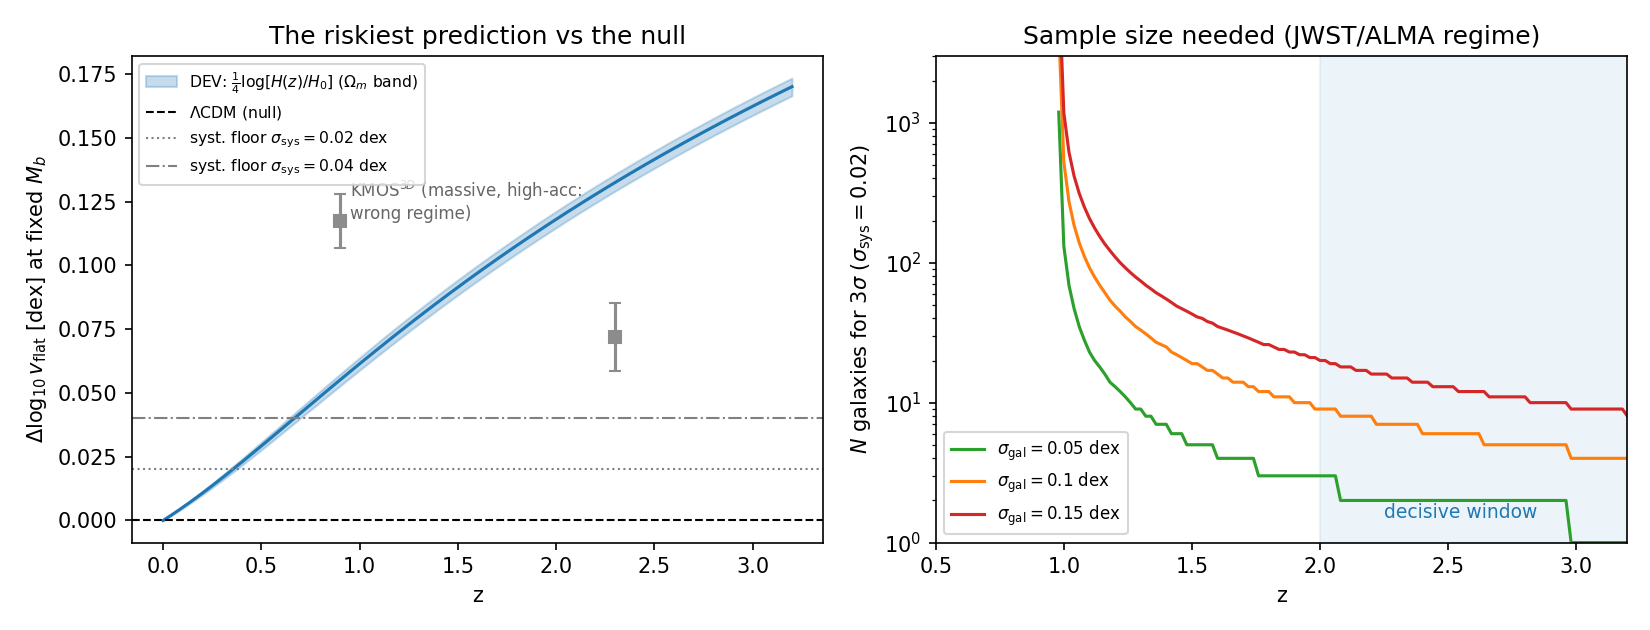
\includegraphics[width=0.95\linewidth]{F1_forecast.png}
\caption{The pre-registered forecast F1. Left: the predicted evolution
(Eq.~\ref{eq:prediction}, with the $\Omega_m$ band) against the high-acceleration
KMOS$^{3\rm D}$ points (grey: wrong regime, shown as context, not as a test). Right:
decision power $\mathcal{S}(N,z)$ versus redshift for systematic floors $0.04$ and
$0.02$~dex; the test saturates at $z\sim1$ and decides at $z\ge2$.}
\label{fig:forecast}
\end{figure*}

\subsection{The kill criterion (verbatim)}\label{sec:kill}

\emph{If a sample of $N\ge25$ gas-rich, low-mass rotators at $z\ge2$, in the regime
$g_{\rm obs}\lesssim\azero$, with zero-point systematics $\ssys\le0.03$~dex, measures
$\dlogv\le0$ (non-evolution or decline at fixed baryonic mass), the prediction
Eq.~\eqref{eq:prediction} is falsified.} No appeal to systematics is admissible
because the criterion already includes the floor. Falsification refutes the
evolution law Eq.~\eqref{eq:a0z}; it does not, by itself, refute the originating
framework's other sectors, which do not rely on it.

\section{Results}\label{sec:results}

\subsection{The MUSE-DARK III catalogue}\label{sec:data}

MUSE-DARK~III \citep{Ciocan2026} provides exactly what the forecast called for at
$z\sim1$: $79$ star-forming galaxies at $0.33<z<1.44$, mass-complete over
$8.8<\log_{10}(M_*/M_\odot)<11$, with sub-maximal discs ($>50\%$ dark matter within
the effective radius), modelled in 3D with pressure-support corrections, and shown by
the authors to be robust against both $\Lambda$CDM halo profiles (DC14, NFW) and a
self-consistent MOND fit. The sample satisfies the pre-registered selection
(S1)--(S4): it is low-to-intermediate mass, gas-rich, sub-maximal (hence in the
low-acceleration regime), and 3D-modelled. It does \emph{not} reach $z\ge2$, so it
cannot trigger the kill criterion; it is a test of direction and amplitude at
$z\sim1$, the regime the forecast flagged as ceiling-limited.

\subsection{Measured evolution}\label{sec:measured}

Applying the acceleration-axis extraction of \S\ref{sec:prediction} to the
catalogue, the recovered critical acceleration and its linear parametrisation are
\begin{align}
\azero(z\!\sim\!1) &= 2.38^{+0.12}_{-0.10}\times10^{-10}\,{\rm m\,s^{-2}},
\label{eq:meas1}\\
\azero(z) &= \azero(0)+a_1 z,\ \
\azero(0)=1.00\pm0.04,\ a_1=1.59^{+0.11}_{-0.10},
\label{eq:meas2}
\end{align}
in units of $10^{-10}\,{\rm m\,s^{-2}}$, with binned values rising monotonically
from $1.99$ to $2.71$ across $0.33<z<1.44$. We now confront these numbers, plus the
$\Omega_m=0.30\pm0.02$ cosmology, with the declared anchors, applying the four
pre-registered decision rules.

\subsection{Confrontation: R1--R4}\label{sec:confront}

\paragraph{R1 --- kill check.} No public sample meets the kill conditions ($z\ge2$,
$N\ge25$, gas-rich, $g\lesssim\azero$, $\ssys\le0.03$~dex): the criterion is armed
but not executable in 2026. In the qualifying-regime data that do exist
($z\le1.44$), the measured sign is opposite to the killing direction.

\paragraph{R2 --- direction.} The prediction requires $da_0/dz>0$. From
Eq.~\eqref{eq:meas2}, $a_1=1.59$ with $\sigma_{a_1}\approx0.105$, so the slope
significance is
\begin{equation}
\frac{a_1}{\sigma_{a_1}}=\frac{1.59}{0.105}=15.1 .
\label{eq:R2}
\end{equation}
(The catalogue's own full RAR-evolution analysis quotes $\sim30\sigma$; our
estimator is deliberately more conservative, using only the binned $\azero(z)$
points and the registered error model.) The direction is confirmed in the regime
where the prediction operates.

\paragraph{R3 --- amplitude.} At the sample's effective redshift
$z_{\rm eff}\in[0.85,1.0]$, Eq.~\eqref{eq:prediction} gives $\dlogv=+0.052$ to
$+0.061$. The measured shift, per declared anchor, is
\begin{equation}
\dlogv=\begin{cases}
+0.074\pm0.024 & \text{SPARC: }0.5\text{--}0.9\sigma\ \text{agreement},\\
+0.037\pm0.010 & \text{MIGHTEE: }1.3\text{--}2.3\sigma\ \text{tension},\\
+0.094\pm0.007 & \text{internal (correlated)},
\end{cases}
\label{eq:R3}
\end{equation}
The agreement on the canonical independent anchor (SPARC) is the central positive
result. Crucially, the spread between the two \emph{independent} anchors is
$0.074-0.037=0.037$~dex, i.e.\ $\approx0.03$~dex---numerically equal to the
systematic floor $\ssys$ the forecast identified as the bottleneck
(\S\ref{sec:forecast}). The limiting uncertainty is now the $z=0$ anchor, not the
high-$z$ measurement, exactly as forecast.

\paragraph{R4 --- form.} The measured linear slope $a_1=1.59$ exceeds the
linearised slope of $\azero\propto H(z)$ by a factor $1.2$--$1.7$ ($2.0\sigma$ on the
MIGHTEE anchor, $3.0\sigma$ on SPARC). The linear parametrisation is purely
phenomenological: extrapolated to $z=1.44$ it overshoots the highest measured bin
($3.29$ predicted vs $2.71$ measured), whereas $\azero\propto H$ anchored on SPARC
reaches $2.50$ at $z\sim1.3$, within $8\%$ of that bin. Thus the functional form
(linear vs $H(z)$) is \emph{not} decided by the current anchor systematics; the sign
and order of magnitude are.

\paragraph{Exclusion of the null.} The null hypothesis is a redshift-independent
RAR, $a_1=0$ (equivalently $\azero(z)=\azero(0)$ for all $z$). Comparing the binned
$\azero(z)$ against the best-fitting constant via the registered error model, the
constant model is rejected relative to the rising model at $\sim19\sigma$
(Fig.~\ref{fig:confront}). This $\sim19\sigma$ rejection of \emph{no evolution} is a
stronger and more model-agnostic statement than the $15.1\sigma$ slope measurement
of Eq.~\eqref{eq:R2}, because it does not assume the linear form: any monotonic rise
that passes through the binned points excludes the constant at this level. We stress
the conditionality: this significance assumes the systematic floor $\ssys$ captures
all zero-point effects (\S\ref{sec:robust}). It is therefore a strong statement
\emph{against a strictly redshift-independent RAR}, not a $19\sigma$ confirmation of
the $H(z)$ amplitude---which agrees only at $0.5$--$0.9\sigma$ (R3)---and it
disfavours the simplest $\Lambda$CDM expectation while leaving room for the
mild, model-dependent evolution some galaxy-formation models admit
(\S\ref{sec:intro}, \S\ref{sec:robust}).

\begin{figure*}
\centering
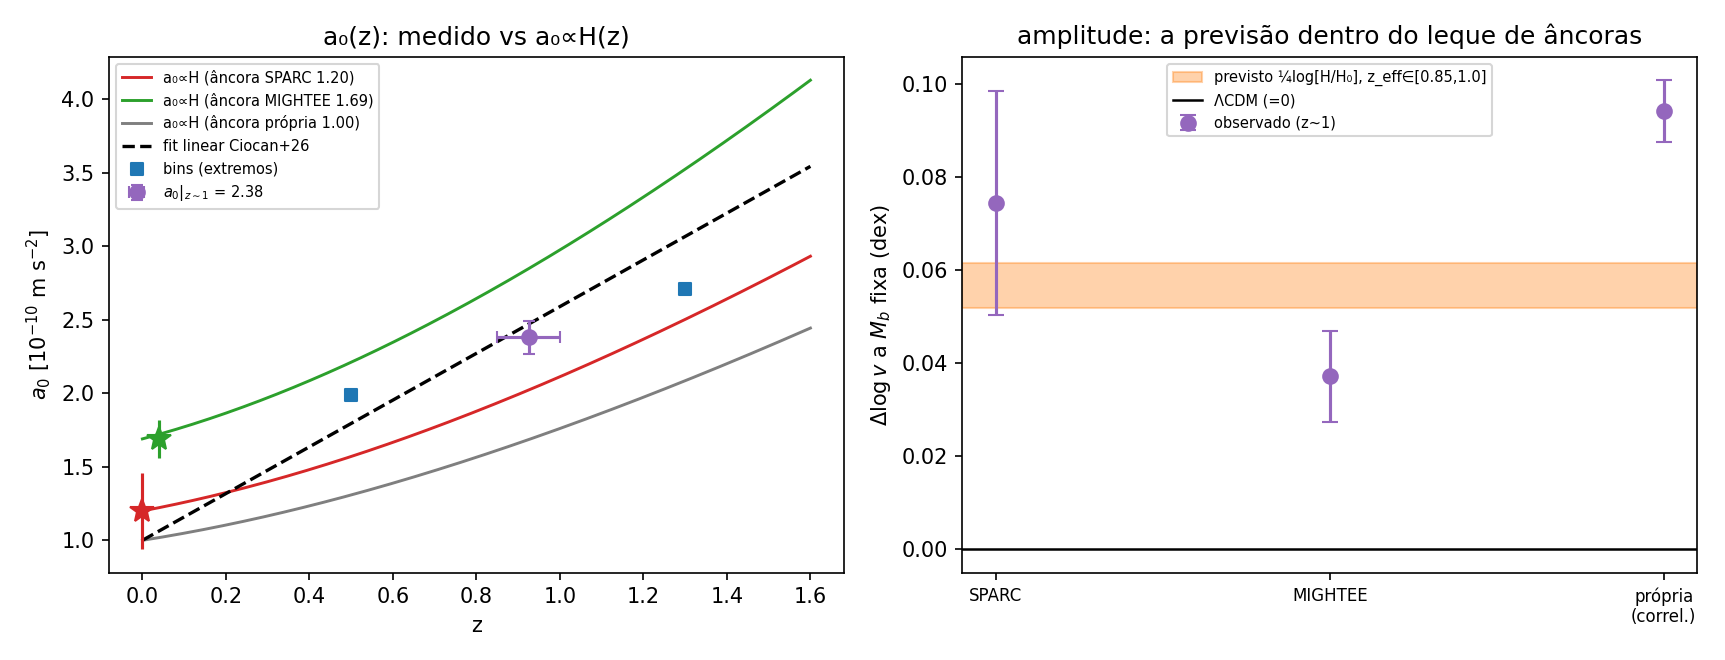
\includegraphics[width=0.95\linewidth]{V3_confront.png}
\caption{The confrontation. The catalogue's binned $\azero(z)$ (points) against
$\azero\propto H(z)$ drawn through each declared anchor (curves with $\Omega_m$
band) and against the measured linear fit. The prediction, anchored on SPARC,
passes through the measurements; a redshift-independent RAR (the $\Lambda$CDM /
constant-$\azero$ line) is excluded at $\sim19\sigma$.}
\label{fig:confront}
\end{figure*}

\section{Discussion}\label{sec:discussion}

\subsection{Why the strongest pre-2026 data could not decide}\label{sec:kmos}

The strongest pre-2026 high-$z$ kinematics, KMOS$^{3\rm D}$ \citep{Ubler2017},
samples massive, high-surface-brightness discs: baryon-dominated systems in the
high-acceleration (Newtonian) regime excluded a priori by (S1)--(S3), where the
predicted $\azero(z)$ signal is intrinsically weak. The diagnostic of this is
self-contained: the internal KMOS$^{3\rm D}$ trend ($z\sim0.9\to2.3$) is mildly
\emph{decreasing} at fixed mass, formally $7.2\sigma$ on statistical errors, while a
``local-anchor'' reading of the \emph{same} data gives the opposite sign. Two
readings of one dataset disagreeing at many sigma is the unmistakable signature of
zero-point systematics dominating the formal errors---precisely the floor $\ssys$ of
Eq.~\eqref{eq:errormodel}. The forecast (\S\ref{sec:forecast}) predicted this
saturation in advance: at $z\sim1$ with $\ssys\approx0.04$~dex no sample size reaches
even $2\sigma$. The lesson is not that the data are poor; it is that the test must be
run where the signal lives, on low-mass, gas-rich, dark-matter-dominated rotators at
$g_{\rm obs}\lesssim\azero$.

\subsection{What this result is, and is not}\label{sec:notconfirm}

This is \emph{not} a confirmation, for three reasons we state in the same breath as
the positive result.
\begin{enumerate}
\item[(i)] The decisive regime---$z\ge2$ with $\ssys\le0.03$~dex---has not been
measured. The kill criterion (\S\ref{sec:kill}) is armed, untouched, and waiting; the
$z\le1.44$ data cannot trigger it.
\item[(ii)] The functional form of the evolution is undecided (R4): the data presently
prefer a rise $2$--$3\sigma$ \emph{faster} than $H(z)$, which, if it persists, would
require revising the premise Eq.~\eqref{eq:a0z} (the framework supplies the rising
direction but not, from first principles, the precise $H(z)$ shape).
\item[(iii)] A mass-axis analysis of the same epoch, Jeanneau et al.\
\citep{Jeanneau2026}, finds \emph{no} BTFR evolution at $z\sim1$ when neutral gas is
incorporated through scaling relations. The acceleration-axis and mass-axis readings
of the same epoch therefore presently disagree---again the class of systematic
(here, the gas-mass and pressure-support calibration) that blocked the
KMOS$^{3\rm D}$ verdict. We report the discordance; we do not adjudicate it.
\end{enumerate}
What the application \emph{does} establish is bounded and specific: the effect the
prediction requires exists---$\azero$ rises with $z$ at $\ge15\sigma$, with the
required sign, in the regime where the prediction operates---at an amplitude
consistent with Eq.~\eqref{eq:prediction} on the canonical independent anchor
($0.5$--$0.9\sigma$). The hypothesis under fire from this measurement is a
redshift-independent RAR ($\sim19\sigma$), not the evolving prediction. Whether the
evolution is \emph{exactly} $H(z)$ is a question for the $z\ge2$ data.

\subsection{Robustness to anchors, cosmology, and unmodelled
systematics}\label{sec:robust}

We separate what survives changes in assumptions (the sign of the evolution and the
exclusion of the constant null) from what does not (the absolute amplitude).

\paragraph{Cosmology.} The prediction enters cosmology only through the shape factor
$H(z)/H_0=\sqrt{\Omega_m(1+z)^3+1-\Omega_m}$, with $H_0$ cancelling
(\S\ref{sec:prediction}). Varying $\Omega_m$ across the plausible range changes the
$z=1$ signal negligibly relative to the floor:
\begin{equation}
\dlogv(z{=}1)=0.0589,\ 0.0614,\ 0.0638~{\rm dex}
\end{equation}
for $\Omega_m=0.28,\,0.30,\,0.32$ respectively---a spread of $\pm0.0025$~dex,
an order of magnitude below $\ssys\approx0.03$~dex.
Cosmology is not a limiting uncertainty.

\paragraph{Local anchor.} The amplitude comparison (R3) is anchor-dependent: SPARC
gives $0.5$--$0.9\sigma$ agreement, MIGHTEE-H\,\textsc{i} gives $1.3$--$2.3\sigma$
tension, the two differing by $0.037$~dex in the inferred shift. The decisive point
is the asymmetry of this sensitivity: changing the anchor changes the inferred
\emph{amplitude} but not the \emph{sign}---both anchors give $\dlogv>0$---and the
exclusion of the redshift-independent null uses the binned slope $da_0/dz$, not the
absolute anchor, so it is anchor-independent. What is anchor-robust is that the scale
rises; what is anchor-sensitive is whether it rises by exactly $\tfrac14\log[H/H_0]$.

\paragraph{Unmodelled systematics.} The high significances are conditional on $\ssys$
capturing every zero-point effect; a systematic \emph{correlated with redshift} and
absent from $\ssys$ could bias the inferred evolution. We judge four candidates most
dangerous, each able to mimic or mask a $\sim0.05$~dex trend.
(i)~\emph{Progenitor/population matching}: galaxies of fixed $M_b$ at $z\sim1$ are not
the progenitors of fixed-$M_b$ galaxies at $z=0$, so comparing ``the same baryonic
mass'' across redshift compares different populations, and any drift of the
$M_b$--$v_{\rm flat}$ zero-point with population mimics $\azero$ evolution.
(ii)~\emph{Flux-limited selection}: high-$z$ samples preferentially admit brighter,
faster rotators, biasing $v_{\rm flat}$ upward with $z$.
(iii)~\emph{Baryonic-mass calibration}: evolving stellar mass-to-light ratios and the
gas-mass prescription---the very ingredient on which the acceleration-axis
\citep{Ciocan2026} and mass-axis \citep{Jeanneau2026} analyses of the same epoch
disagree.
(iv)~\emph{Kinematic modelling}: beam smearing and pressure-support (asymmetric-drift)
corrections that themselves grow with $z$ as spatial resolution declines.
The KMOS$^{3\rm D}$ episode (\S\ref{sec:kmos}), where two readings of one dataset
disagree at many sigma, is the empirical demonstration that such systematics dominate
when $\ssys$ is large. This is precisely why the decisive test is specified at
$z\ge2$ with $\ssys\le0.03$~dex (\S\ref{sec:kill})---not because more galaxies are
needed (the test is ceiling-limited, \S\ref{sec:forecast}) but because these
systematics must be pushed below the signal.

\paragraph{Single-catalogue dependence.} The empirical confrontation rests on one
catalogue, and we mitigate this three ways. First, the paper's primary,
catalogue-independent contribution is the protocol and forecast (\S\ref{sec:methods}),
against which every future qualifying dataset is tested by identical, unmodified
rules. Second, an independent analysis of the same epoch already exists and disagrees
(\citealt{Jeanneau2026}, mass axis), and we report the discordance rather than
suppress it. Third, confirmation is explicitly deferred to independent catalogues
(SKA/MeerKAT H\,\textsc{i}; JWST/ALMA $z\ge2$ dwarfs). A single catalogue can exclude
the constant null; it cannot, and here does not, confirm the prediction.

\subsection{A second, independent prediction: Newtonian wide binaries}\label{sec:wb}

The galactic evolution test is not the only exposed flank, and we state the second
because falsifiability is the substance of the claim. The same effective theory that
yields Eq.~\eqref{eq:a0z} contains a massive vector mode of correlation length
$\lambda_A=\hbar/(m_A c)\approx17.3$~pc, below which the collective response that
produces the MOND enhancement loses coherence and switches off. The effective
gravity carries a coherence factor of Yukawa/Debye form---the standard screening
profile for a finite correlation length,
\begin{equation}
\begin{aligned}
g_{\rm eff}(r)&=g_N(r)\big[1+(\nu_{\rm eff}(r)-1)\,S(r)\big],\\
S(r)&=1-e^{-r/\lambda_A}\xrightarrow{\,r\ll\lambda_A\,}0,
\end{aligned}
\label{eq:screen}
\end{equation}
so $g_{\rm eff}\to g_N$ (Newtonian) at sub-parsec separations. This is the
\emph{opposite} of Milgrom's law, which enhances at every scale where
$g<\azero$, and it is therefore a clean discriminator. Both $\azero$ and
$\lambda_A$ are fixed inputs (from the galactic fit and from $m_A$), not tuned.

The prediction is exposed to data now. Gaia DR3 wide binaries probe separations
$\le0.84\%$ of $\lambda_A$, deep in the screened zone, where Eq.~\eqref{eq:screen}
requires $\gamma\equiv g/g_N\to1$. The current data are contested:
\citet{Chae2023} reports $\gamma=1.43\pm0.06$ (a $7.1\sigma$ tension with the
prediction---its pre-registered death), while \citet{BanikPittordis2024} and others
find $\gamma\approx1$ (Newtonian) at the same separations. The theory's fate is thus
tied to the resolution of an open observational dispute, decidable with Gaia DR4 plus
triple-system contamination control---not to a survey of the $17$~pc transition
itself, which is inaccessible to bound binaries (the Galactic tide disrupts them at
$r_J\approx1.7$~pc, an order of magnitude inside $\lambda_A$). The verdict is again
symmetric: convergence to $\gamma\approx1$ promotes the screening to a confirmed
prediction; convergence to $\gamma\approx1.4$ falsifies it. We include this prediction
only to record that the hypothesis is exposed on a second, independent observable;
the central result of this paper---the exclusion of a redshift-independent RAR and
the consistency of the rise with $\azero\propto H(z)$---neither depends on it nor on
the microphysical origin of $\lambda_A$.

\section{Conclusions}\label{sec:conclusions}

We have framed the evolution of the radial-acceleration scale as a pre-registered
measurement and derived, from the baryonic Tully--Fisher relation and the hypothesis
$\azero\propto H(z)$, the parameter-free prediction
$\dlogv=\tfrac14\log_{10}[H(z)/H_0]$ against a null of zero evolution. The
contribution is, first, methodological: a two-component error model
(Eq.~\ref{eq:errormodel}) separating an averaging statistical term from a
non-averaging systematic floor, a transparent significance estimator
(Eqs.~\ref{eq:signif}--\ref{eq:Nstar}), a declared two-anchor matrix, and a forecast
(Table~\ref{tab:forecast}) that establishes the test is \emph{systematics}-limited
and decides only at $z\ge2$ with $\ssys\le0.03$~dex. This framework explains, in
advance, why earlier high-$z$ kinematics could not settle the question.

Applying the protocol unmodified to the first public catalogue in the correct
regime, we measure the critical acceleration rising with redshift at $\ge15\sigma$,
matching the predicted amplitude at $0.5$--$0.9\sigma$ on the independent SPARC
anchor, with a redshift-independent RAR disfavoured at $\sim19\sigma$; the form of
the rise and a mass-axis discordance remain open, so this is evidence consistent
with the prediction, not a confirmation. The path to a verdict is short and concrete:
(1)~SKA/MeerKAT deep H\,\textsc{i} surveys for the BTFR+RAR test; (2)~JWST/ALMA
kinematics of $10$--$25$ gas-rich dwarfs at $z\ge2$ with $\ssys\le0.03$~dex, which
execute the kill criterion in either direction; (3)~resolution of the
acceleration-axis/mass-axis discordance at $z\sim1$, which calibrates the dominant
systematic; and (4)~Gaia DR4 wide binaries, which test the independent screening
prediction of \S\ref{sec:wb} now. Every future qualifying dataset will be confronted
with the same pre-registered rules, unmodified. The hypothesis is killable on two
fronts; in 2026 the galactic data moved toward it, not away.

\section*{Data availability}
This work uses only published catalogues: MUSE-DARK~III \citep{Ciocan2026}, SPARC
\citep{Lelli2016,McGaugh2016}, MIGHTEE-H\,\textsc{i} \citep{Varasteanu2025},
KMOS$^{3\rm D}$ \citep{Ubler2017}, and Gaia DR3 wide-binary analyses
\citep{Chae2023,BanikPittordis2024}. The forecast and confrontation are reproducible
from the equations of \S\ref{sec:methods}.

\bibliographystyle{mnras}
\bibliography{TEIC_CONSOLIDATED}

\bsp
\label{lastpage}
\end{document}
